\documentclass[tikz,border=2pt]{standalone}
\usepackage{pgfplots}
\usepgfplotslibrary{groupplots}
\pgfplotsset{compat=1.18}
\definecolor{blue}{HTML}{0072B2}\definecolor{sky}{HTML}{56B4E9}
\definecolor{green}{HTML}{009E73}\definecolor{orange}{HTML}{E69F00}
\definecolor{verm}{HTML}{D55E00}\definecolor{ink}{HTML}{263238}
\begin{document}
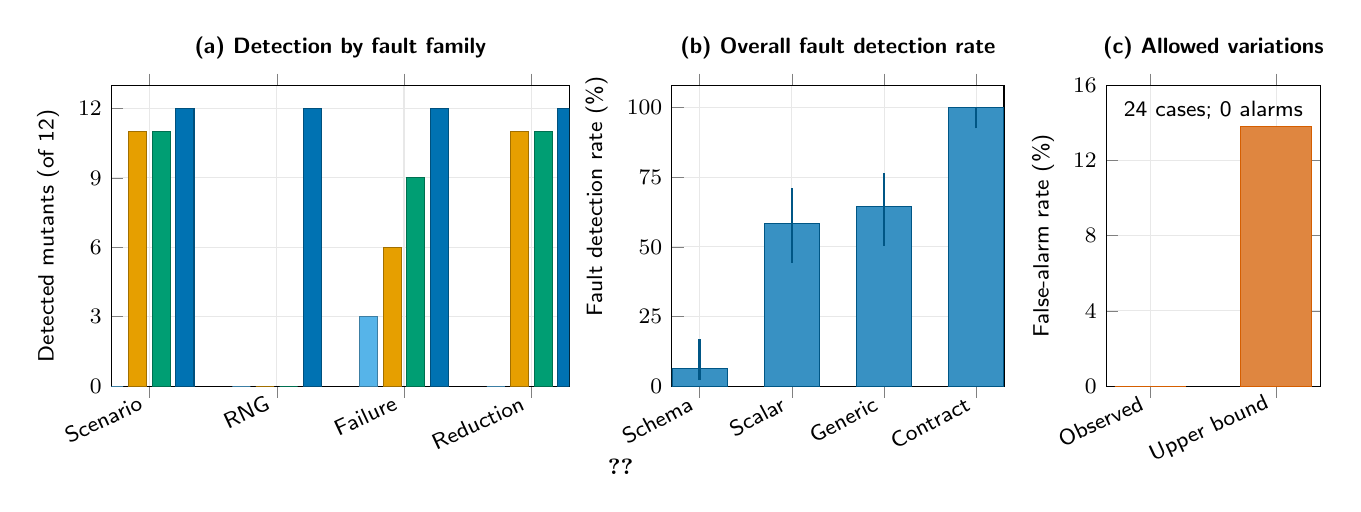
\begin{tikzpicture}[font=\sffamily\fontsize{8}{9.2}\selectfont]
\begin{groupplot}[group style={group size=3 by 1,horizontal sep=13mm},height=54mm,
  tick label style={font=\sffamily\fontsize{8}{9}\selectfont},
  label style={font=\sffamily\fontsize{8}{9}\selectfont},
  title style={font=\sffamily\bfseries\fontsize{8}{9}\selectfont},
  legend style={font=\sffamily\fontsize{8}{9}\selectfont,draw=none,fill=none,/tikz/every even column/.append style={column sep=3mm}}]
\nextgroupplot[title={(a) Detection by fault family},width=74mm,ybar,bar width=2.3mm,
  symbolic x coords={Scenario,RNG,Failure,Reduction},xtick=data,xticklabel style={rotate=25,anchor=east},
  ymin=0,ymax=13,ytick={0,3,6,9,12},ylabel={Detected mutants (of 12)},grid=major,grid style={gray!18},
  legend columns=2,legend to name=detlegend]
\addplot[fill=sky,draw=sky!70!black] coordinates {(Scenario,0)(RNG,0)(Failure,3)(Reduction,0)};
\addlegendentry{Schema}
\addplot[fill=orange,draw=orange!70!black] coordinates {(Scenario,11)(RNG,0)(Failure,6)(Reduction,11)};
\addlegendentry{Scalar}
\addplot[fill=green,draw=green!70!black] coordinates {(Scenario,11)(RNG,0)(Failure,9)(Reduction,11)};
\addlegendentry{Generic}
\addplot[fill=blue,draw=blue!70!black] coordinates {(Scenario,12)(RNG,12)(Failure,12)(Reduction,12)};
\addlegendentry{Contract}

\nextgroupplot[title={(b) Overall fault detection rate},width=58mm,ybar,bar width=7mm,
  symbolic x coords={Schema,Scalar,Generic,Contract},xtick=data,xticklabel style={rotate=28,anchor=east},
  ymin=0,ymax=108,ytick={0,25,50,75,100},ylabel={Fault detection rate (\%)},ylabel style={xshift=5mm},grid=major,grid style={gray!18}]
\addplot[draw=blue!75!black,fill=blue!78] coordinates {(Schema,6.250)(Scalar,58.333)(Generic,64.583)(Contract,100)};
\draw[blue!75!black,line width=.8pt] (axis cs:Schema,2.148)--(axis cs:Schema,16.835);
\draw[blue!75!black,line width=.8pt] (axis cs:Scalar,44.281)--(axis cs:Scalar,71.150);
\draw[blue!75!black,line width=.8pt] (axis cs:Generic,50.439)--(axis cs:Generic,76.566);
\draw[blue!75!black,line width=.8pt] (axis cs:Contract,92.590)--(axis cs:Contract,100);

\nextgroupplot[title={(c) Allowed variations},width=43mm,ybar,bar width=9mm,
  symbolic x coords={Observed,Upper bound},xtick=data,xticklabel style={rotate=25,anchor=east},
  enlarge x limits=0.35,ymin=0,ymax=16,ytick={0,4,8,12,16},ylabel={False-alarm rate (\%)},grid=major,grid style={gray!18}]
\addplot[fill=verm!75,draw=verm] coordinates {(Observed,0)(Upper bound,13.798)};
\node[anchor=north,font=\sffamily\fontsize{8}{9}\selectfont] at (rel axis cs:.5,.98) {24 cases; 0 alarms};
\end{groupplot}
\node[anchor=north] at ($(group c1r1.south east)!0.5!(group c2r1.south west)+(0,-8mm)$) {\ref{detlegend}};
\end{tikzpicture}
\end{document}
